\chapter{Dataset Construction and Labeling}\label{ch:dataset}

This chapter describes how the dataset used in this thesis was generated, labelled, and stored. Since the performance of the classification models depends strongly on the diversity and quality of the recorded insertion attempts, the dataset generation was treated as a central methodological part of the work.

\section{Data Collection Procedure}\label{sec:dataset_collection}

All data was recorded on the real robotic system described in \chapref{ch:rob_setup}. Each sample corresponds to one insertion attempt of one rod into one hole under a defined set of deviations. During each cycle, the robot grasped one of the rods from the dedicated holder, moved to the selected insertion pose above the corresponding hole, performed the insertion under force control, and if the insertion was successful pulled the rod back out and released it in its holder or if the insertion failed, released the rod (opened gripper) where it failed, requiring for manual intervention to place the rod back in its holder.

The dataset was generated in three recording batches. In the first recording batch, 100 insertions for each of the nine holes were recorded, resulting in 900 samples in total. This first batch had random positional and angular deviations applied, while other experimental factors were kept fixed. The positional deviation was generated in polar coordiantes by sampling a random radius in a range from [$0.0$, \texttt{max\_radius}] mm, with a random angle range from [$0.0$, $2\pi$] rad. Angular deviations were applied randomly in a range from [-\texttt{min\_max\_devi}, \texttt{min\_max\_devi}] rad around the TCP's $x$- and $y$-axis.
\figref{fig:batch1_example} shows the time series plot of all insertions marked as success in green and fail in red of the first batch on \texttt{rect\_rod\_t0.2}.

\begin{figure}[H]
    \centering
    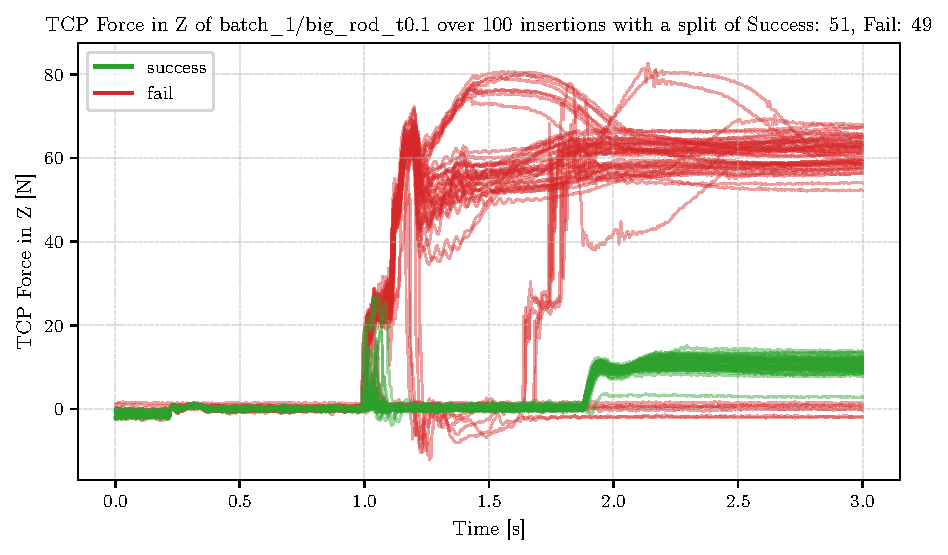
\includegraphics[width=0.75\textwidth]{chapters/4-dataset_construction_and_labeling/SF_batch_1_big_rod_t01.pdf}
    \caption{Time series plot of \texttt{big\_rod\_t0.1} from Batch 1 with 100 insertions, showing individual success and failed force curves.}
    \label{fig:batch1_example}
\end{figure}

For the second and third recording batches, the data collection strategy was redesigned and made systematic, meaning deterministic and not random within bounds as before. First, the dataset should include a broader, more controlled variety of insertion configurations. Which consequently required more attempts per run to cover the full range of possibilities and more time. Typically took one recording session about 1 to 1.5 hours. Second, these long recording runs should be resumable in a reproducible manner without losing track of which settings had already been recorded.

The systematic recording plan was built around three main factors: grasp height, approach height, and insertion force level. Grasp height describes the height at which the rod is grasped from the rod holder. Two grasp heights are used (\SIlist{0.0;7.0}{\milli\meter}), which influences the rods stability in the gripper. At position $0.0$ mm the rod is more stable than position $7.0$ mm, where is rod is grasped more towards the tip. Two approach heights (\SIlist{-5.0;2.0}{\milli\meter}) are used which alter the height above the hole before insertion. Three force levels (\SIlist{15;25;35}{\newton}) are used which specify the UR force mode's target force along the $z$-axis. These factors result in
\begin{equation}
    2 \times 2 \times 3 = 12
    \label{eq:combs_per_hole}
\end{equation}

main combinations per hole. For tight holes, 40 insertion attempts were recorded for each of these combinations, which resulted in
\begin{equation}
    12 \times 40 = 480
    \label{eq:insertions_tight}
\end{equation}
samples per hole. For non-tight holes, i.e.\ the medium and loose tolerances, 30 insertion attempts were recorded per combination, which resulted in
\begin{equation}
    12 \times 30 = 360
    \label{eq:insertions_nontight}    
\end{equation}

samples per hole.

In addition to these three main factors, each insertion attempt was assigned a deterministic deviation state. This deviation state contains one position, orientation, force limit and record offset. The position relative to the holes center is generated in polar coordinates with a radius and angle. The radius is sampled linearly in a range from $0.0$ mm to $0.3$ mm in three steps. Each radius is combined with four angles, them being $0^\circ,90^\circ,180^\circ,270^\circ$, resulting in $3\times 4 = 12$ positional offset states. Note that position $(0,0)$ appears four times, which closer represents reality, when insertions happen successful more often.\\
The orientational tilt around the tools $x$- and $y$-axes was varied using the values \(-3^\circ\), \(0^\circ\), and \(3^\circ\) arranged in a $3\times3$ grid, resulting in $9$ tilt combinations. The force limit for aborting an insertion was cycled through \SIlist{30;40;50}{\newton}, and the recording offset was cycled through \SIlist{-0.2;0.0;0.3;0.6;0.9}{\second}, which starts the recording of data $0.2$ s after or up to $0.9$ s before an insertion was started, which introduced temporal variation into the dataset. As a result, the later batches were no longer purely random, but followed a deterministic, pseudorandom and reproducible recording schedule. This means that the dataset was not a full cartesian sweep over all factors, but it still ensured broad and repeatable coverage of the relevant operating conditions. \figref{fig:create_plan_periodic_bars} shows visually how position, orientation, force limit and record offset are periodially samples along the $30$ or $40$ insertions.

\usetikzlibrary{calc}

% -----------------------------------------
% Figure
% -----------------------------------------
\begin{figure}[htbp]
    \centering
    \begin{tikzpicture}[x=0.33cm,y=0.9cm,font=\small]
        \def\n{40}

        % Row macro:
        % #1 = y-bottom
        % #2 = row label
        % #3 = period m_i
        % #4 = color/style
        \newcommand{\periodrow}[4]{%
            \pgfmathtruncatemacro{\m}{#3}%
            \pgfmathtruncatemacro{\full}{int(\n/\m)}%
            \pgfmathtruncatemacro{\lastfull}{\full-1}%
            \pgfmathtruncatemacro{\rem}{mod(\n,\m)}%

            % horizontal borders of the band
            \draw (0,#1) -- (\n,#1);
            \draw (0,#1+1) -- (\n,#1+1);

            % left label
            \node[left=8pt, align=right] at (0,#1+0.5) {#2};

            % left boundary
            \draw[thick] (0,#1) -- (0,#1+1);

            % full separators
            \foreach \k in {1,...,\full} {
                \pgfmathsetmacro{\xk}{\k*\m}
                \draw[#4,thick] (\xk,#1) -- (\xk,#1+1);
            }

            % labels for full segments
            \foreach \k in {0,...,\lastfull} {
                \pgfmathsetmacro{\xa}{\k*\m}
                \pgfmathsetmacro{\xb}{(\k+1)*\m}
                \node[#4] at ({(\xa+\xb)/2},{#1+0.5}) {\(\m\)};
            }

            % remainder segment, if any
            \ifnum\rem>0
                \pgfmathsetmacro{\xa}{\full*\m}
                \draw[#4,thick] (\n,#1) -- (\n,#1+1);
                \node[#4] at ({(\xa+\n)/2},{#1+0.5}) {\(\rem\)};
            \fi
        }

        % left spine
        \draw[thick] (0,0) -- (0,4.45);

        % top count line
        \draw[thick] (0,4) -- (\n,4);
        \node[above left] at (0,4.15) {$12\times$};

        % small ticks on top line
        \foreach \x in {0,...,40}{
            \draw (\x,4) -- (\x,4.07);
        }

        % top labels
        \foreach \i in {1,5,10,15,20,25,30,35,40}{
            \node[above] at ({\i-0.5},4.07) {\i};
        }

        % rows
        \periodrow{3}{Position}{12}{red!75!black}
        \periodrow{2}{Tilt}{9}{red!75!black}
        \periodrow{1}{Force limit}{3}{red!75!black}
        \periodrow{0}{Record offset}{5}{red!75!black}
    \end{tikzpicture}
    \caption{Periodic modulation scheme used in \texttt{create\_plan()} for one 40-sample block. The four deviations are generated with periods \(m_i \in \{12,9,3,5\}\). For the complete recording plan, this 40-sample block is repeated 12 times based on \equref{eq:combs_per_hole}}
    \label{fig:create_plan_periodic_bars}
\end{figure}

The function \texttt{create\_plan()} generats this schedule before the recording run started. The detailed executing can be seen in \algoref{alg:create_plan}.

% In document
\begin{algorithm}[htbp]
\caption{\texttt{create\_plan()} for systematic dataset generation}
\label{alg:create_plan}
\begin{algorithmic}[1]
\State $\texttt{plan} \gets [\ ]$
\State $\texttt{radius\_steps} \gets$ equally spaced list of length \texttt{pos\_steps} from \texttt{pos\_min} to \texttt{pos\_max} (here: 3 values from \SI{0.0}{\milli\meter} to \SI{0.3}{\milli\meter})
\State $\texttt{angle\_steps} \gets$ equally spaced list of length \texttt{ang\_steps} from \(0\) to \(2\pi\), excluding the endpoint (here: 4 angular directions)
\State $\texttt{tilt\_combinations} \gets$ all combinations of \texttt{tilt\_x} and \texttt{tilt\_y} from \texttt{tilt\_list\_rad} (here: \(3\times 3 = 9\) combinations)

\ForAll{$\texttt{gh} \in \texttt{grasp\_heights\_mm}$}
    \ForAll{$\texttt{ah} \in \texttt{approach\_heights\_mm}$}
        \ForAll{$\texttt{fl} \in \texttt{force\_levels}$}

            \If{\texttt{tolerance} is tight}
                \State $\texttt{n} \gets \texttt{num\_insertions\_tight}$ \Comment{here: 40}
            \Else
                \State $\texttt{n} \gets \texttt{num\_insertions\_not\_tight}$ \Comment{here: 30}
            \EndIf

            \For{$i = 0$ to $\texttt{n}-1$}
                \State \texttt{angle} $\gets$ \texttt{angle\_steps}[$i \mod$ len(\texttt{angle\_steps})]
                \State \texttt{radius} $\gets$ \texttt{radius\_steps}[floor($i$ / len(\texttt{angle\_steps})) $\mod$ len(\texttt{radius\_steps})]
                \State $\texttt{devi} \gets (\texttt{radius}\cos(\texttt{angle}),\texttt{radius}\sin(\texttt{angle}))$
                \State \texttt{tilt} $\gets$ \texttt{tilt\_combinations}[$i \mod$ len(\texttt{tilt\_combinations})]
                \State \texttt{f\_limit} $\gets$ \texttt{force\_limits}[$i \mod$ len(\texttt{f\_limit})]
                \State \texttt{record\_offset} $\gets$ \texttt{record\_offset\_s}[$i \mod$ len(\texttt{record\_offset\_s})]
                \State append $(\texttt{gh},\texttt{ah},\texttt{fl},\texttt{devi},\texttt{tilt},\texttt{f\_limit},\texttt{record\_offset})$ to \texttt{plan}
            \EndFor

        \EndFor
    \EndFor
\EndFor

\State \Return \texttt{plan}
\end{algorithmic}
\end{algorithm}

\figref{fig:batch2_example} shows exemplary the result of applying more diversity to the dataset for Batch 2 and Batch 3.

\begin{figure}[H]
    \centering
    \includegraphics[width=0.75\textwidth]{chapters/4-dataset_construction_and_labeling/SF_batch_2_big_rod_t01.pdf}
    \caption{Time series plot of \texttt{big\_rod\_t0.1} from Batch 2 with 480 insertions, showing individual success and failed force curves.}
    \label{fig:batch2_example}
\end{figure}

The robot trajectory itself was also optimized to reduce unnecessary waiting and travel time between insertions. In successful insertions, one full cycle typically took about \SI{5}{\second}. In failed insertions, the cycle time increased to approximately \SIrange{8}{10}{\second}, because the rod had to be placed back manually into the robot holder before the next attempt could start.

The insertion was executed using the UR force mode. After the robot reached the pose above the target hole, the force/torque sensor was zeroed and the force controller was configured with a damping value of $0.1$ and a gain scaling of $1.2$. The task frame was defined at the insertion pose. In the final recording implementation, the selection vector was set to
\begin{equation}
    [0,0,1,0,0,0],
    \label{eq:force_mode_selection_vector}
\end{equation}
which means that only the translational $z$-axis was compliant while the remaining axes were kept position-controlled. The applied wrench was
\begin{equation}
    [0,0,F_z,0,0,0],
    \label{eq:force_mode_wrench_vector}
\end{equation}

where $F_z$ corresponds to the selected force level of the current trial. The force-mode limits were set to
\begin{equation}
    [0.001, 0.001, 0.08, 0.8, 0.8, 0.2].
    \label{eq:force_mode_limits_vector}
\end{equation}
For compliant axes, these values are the maximum allowed tcp speed in $m/s$ or $rad/s$ along/about the axis. For non-compliant axes, these values are the maximum allowed deviation along/about an axis between the actual tcp position and the one set by the program.\cite{ur-rtde-api}

Another important design choice concerned the sequence timing. Once a success or failure condition has been detected, the insertion motion was stopped, but the recording was not terminated immediately. Instead, the program continued recording until the full predefined sequence length of \SI{3.0}{\second} has been reached. This was necessary to avoid label leakage through sequence length. Otherwise, the machine learning model could potentially distinguish successful and failed insertions simply based sequence length, rather than based on the actual signal content.

\section{Success and Failure Labeling}\label{sec:dataset_labeling}

The labeling procedure was performed online during data collection. No manual post-hoc annotation of successful and failed insertions was required. The mechanical principle of success detection has already been explained in Chapter~\ref{ch:rob_setup}. From the software perspective, an insertion attempt was labelled as successful when the measured load-cell value exceeded a threshold of 30\,000 during the insertion process. Once this threshold was reached, the motion was stopped and the current sequence was marked as a successful insertion.

All remaining attempts were labelled as failures. In order to preserve additional information about the failure mode, three different failure reasons were stored in the metadata. The first failure condition is a timeout. This occurred when no successful insertion has been detected before the predefined sequence length of \SI{3.0}{\second} has elapsed. The second failure condition is a stall or jam. This was detected when the absolute TCP velocity in insertion direction fell below \SI{0.002}{\meter\per\second} while the absolute force in $z$-direction exceeded \SI{15}{\newton} for more than \SI{0.25}{\second}. The third failure condition is an exceeded force limit. In this case, if the measured force in insertion direction became larger than the force limit defined for the current trial, the insertions label is marked as failure due to force limit reached. Especially for this case recording continued until the fixed sequence length of \SI{3}{\second} is reached. Depending on the plan item, this threshold was set to \SI{30}{\newton}, \SI{40}{\newton}, or \SI{50}{\newton}.

\section{Dataset Composition and Storage}\label{sec:dataset_composition}

For each recorded insertion attempt, 48 robot signals were sampled at \SI{500}{\hertz}, UR's Real-Time Data Exchange (RTDE) maximum poll rate\cite{ur-rtde-guide}. Since each sequence has a fixed length of \SI{3.0}{\second}, each sequence contains 1500 time sampels. One insertion attempt was saved as one CSV file containing the time series data and one JSON file containing the associated metadata. Both files shared the same basename and followed the naming scheme \texttt{sample\_\{n\}\_session\_\{m\}}.

The sample index $n$ denotes the running insertion number, while the session index $m$ denotes the recording session. The session number was increased whenever a recording run was interrupted and later resumed, for example after changing settings or taking a break. This was particularly useful for the longer systematic recordings, because it allowed the collection process to resume from the current point in the plan without overwriting existing files.

Each CSV file is approximately \SI{770}{\kilo\byte} in size and stores the full recorded multivariate time series. The recorded signals are summarized in \tabref{tab:recorded_signals}.

\begin{table}[htbp]
    \centering
    \caption{Recorded signals stored for each insertion attempt.}
    \label{tab:recorded_signals}
    \begin{tabular}{lll}
        \hline
        Signal group & Count & Unit / description \\
        \hline
        Timestamp & 1 & time since start of sequence [s] \\
        TCP force/torque wrench & 6 & forces [N], torques [Nm] \\
        TCP pose & 6 & position [m], orientation [rad] \\
        TCP velocity & 6 & linear [m/s], angular [rad/s] \\
        Joint positions \(q\) & 6 & joint angles [rad] \\
        Joint velocities \(\dot{q}\) & 6 & joint velocities [rad/s] \\
        Tool accelerometer & 3 & Cartesian tool acceleration [m/s\(^2\)] \\
        Robot current & 1 & total robot current [A] \\
        Robot voltage & 1 & total robot voltage [V] \\
        Joint currents & 6 & motor current per joint [A] \\
        Joint temperatures & 6 & joint temperature per joint [\(^\circ\)C] \\
        \hline
        Total & 48 & -- \\
        \hline
    \end{tabular}
\end{table}

Besides the recorded time series, a JSON metadata file was stored for each insertion. This metadata links the recorded sequence to its generation context and label. In particular, it contains the time of recording, storage location, corresponding CSV file, sampling configuration, sequence length, the complete plan item (applied deviations) of the current trial, the binary success label, the failure reason if applicable, the rod type used (insertion task), the tolerance level, the relevant robot poses, and the measured cycle time. An overview is given in Table~\ref{tab:recorded_metadata}.

\begin{table}[htbp]
    \centering
    \caption{Metadata stored for each recorded insertion attempt.}
    \label{tab:recorded_metadata}
    \begin{tabular}{ll}
        \hline
        Metadata field & Description \\
        \hline
        \texttt{saved\_at} & timestamp of file creation \\
        \texttt{saved\_in} & target folder of the sample \\
        \texttt{corresponding\_csv} & path of the associated CSV file \\
        \texttt{sample\_rate\_Hz} & sampling rate \\
        \texttt{sample\_deltatime\_s} & time between samples \\
        \texttt{num\_samples} & number of recorded time steps \\
        \texttt{num\_insertions} & total number of planned insertions \\
        \texttt{sequence\_length\_s} & saved sequence length \\
        \texttt{plan\_item.grasp\_height} & selected grasp height \\
        \texttt{plan\_item.approach\_height} & selected approach height \\
        \texttt{plan\_item.force\_level} & selected insertion force level \\
        \texttt{plan\_item.force\_limit} & selected abort force threshold \\
        \texttt{plan\_item.record\_offset} & temporal offset of recording start \\
        \texttt{plan\_item.deviation} & Cartesian positional deviation \\
        \texttt{plan\_item.tilt} & angular deviation in tool $x$- and $y$-axes \\
        \texttt{successful\_insertion} & binary success label \\
        \texttt{failure\_reason} & timeout, stall/jam, or force limit \\
        \texttt{insertion\_task} & rod type \\
        \texttt{tolerance} & tolerance level of the current hole \\
        \texttt{holderPose\_Up}, \texttt{holderPose\_Down} & grasping poses \\
        \texttt{insertionPose} & nominal insertion pose \\
        \texttt{cycle\_time\_s} & measured cycle duration \\
        \hline
    \end{tabular}
\end{table}

In terms of dataset size, the first recording batch contains 900 insertion attempts. For the later systematic batches, each batch contains 3 tight holes with 480 samples each and 6 non-tight holes with 360 samples each, resulting in
\begin{equation}
    3 \times 480 + 6 \times 360 = 3600
    \label{eq:big_dataset_size}
\end{equation}
samples per batch. In total a two systematic batches were recorded. Thus, the total dataset size amounts to
\begin{equation}
    900 + 3600 + 3600 = 8100
    \label{eq:total_dataset_size}
\end{equation}
samples.

Class balance was not enforced perfectly, but an approximately balanced distribution between successful and failed insertions was targeted. \tabref{tab:all_batches_classbalance} shows the class balance from all batches and the whole dataset. It can be seen that the balance differs slightly between holes, which reflects the fact that some geometries and tolerances are inherently easier or harder than others. Nevertheless, the batch remains sufficiently balanced overall for the intended binary classification task.

\begin{table}[htbp]
    \centering
    \caption{Class balance of the three recording batches and of the complete dataset.}
    \label{tab:all_batches_classbalance}
    \begin{adjustbox}{max width=\textwidth}
    \begin{tabular}{lrrrrrrrrrrrr}
        \toprule
        & \multicolumn{3}{c}{Batch 1} 
        & \multicolumn{3}{c}{Batch 2} 
        & \multicolumn{3}{c}{Batch 3}
        & \multicolumn{3}{c}{Overall dataset} \\
        \cmidrule(lr){2-4} \cmidrule(lr){5-7} \cmidrule(lr){8-10} \cmidrule(lr){11-13}
        Dataset subset & Success & Failure & Total & Success & Failure & Total & Success & Failure & Total & Success & Failure & Total \\
        \midrule
        \texttt{big\_rod\_t0.1}   & 51 & 49 & 100 & 255 & 225 & 480 & 258 & 222 & 480 & 564 & 496 & 1060 \\
        \texttt{big\_rod\_t0.2}   & 50 & 50 & 100 & 193 & 167 & 360 & 208 & 152 & 360 & 451 & 369 & 820 \\
        \texttt{big\_rod\_t0.3}   & 50 & 50 & 100 & 194 & 166 & 360 & 189 & 171 & 360 & 433 & 387 & 820 \\
        \texttt{small\_rod\_t0.1} & 53 & 47 & 100 & 310 & 170 & 480 & 265 & 215 & 480 & 628 & 432 & 1060 \\
        \texttt{small\_rod\_t0.2} & 48 & 52 & 100 & 230 & 130 & 360 & 236 & 124 & 360 & 514 & 306 & 820 \\
        \texttt{small\_rod\_t0.3} & 41 & 59 & 100 & 196 & 164 & 360 & 158 & 202 & 360 & 395 & 425 & 820 \\
        \texttt{rect\_rod\_t0.1}  & 67 & 33 & 100 & 224 & 256 & 480 & 230 & 250 & 480 & 521 & 539 & 1060 \\
        \texttt{rect\_rod\_t0.2}  & 70 & 30 & 100 & 200 & 160 & 360 & 189 & 171 & 360 & 459 & 361 & 820 \\
        \texttt{rect\_rod\_t0.3}  & 54 & 46 & 100 & 174 & 186 & 360 & 199 & 161 & 360 & 427 & 393 & 820 \\
        \midrule
        Total & 484 & 416 & 900 & 1976 & 1624 & 3600 & 1932 & 1668 & 3600 & 4392 & 3708 & 8100 \\
        \bottomrule
    \end{tabular}
    \end{adjustbox}
\end{table}

\newpage
\section{Preprocessing}\label{sec:dataset_preprocessing}

As the aim of this work was to create a real-world insertion dataset, no filtering, smoothing, trimming, or feature extraction was applied before saving the data. The recorded time series were stored in their original sampled form, apart from one necessary physical correction step.

This correction concerned the measured TCP wrench. Although the robot provides the force and torque values at the TCP, the rotation is still expressed in the robot's base frame\cite{ur-force-torque}. In order to obtain force signals that are physically meaningful with respect to the current tool orientation, the wrench was transformed after recording using the measured TCP pose of each time step. Let

\begin{equation}
    {}^{B}\mathbf{w}_i =
    \begin{bmatrix}
    F_{x,i} & F_{y,i} & F_{z,i} & T_{x,i} & T_{y,i} & T_{z,i}
    \end{bmatrix}^{\mathsf T}
    \label{eq:wrench_1}
\end{equation}

denote the recorded wrench of sample \(i\) in base-frame coordinates, and let

\begin{equation}
    \mathbf{p}_i =
    \begin{bmatrix}
    x_i & y_i & z_i & r_{x,i} & r_{y,i} & r_{z,i}
    \end{bmatrix}^{\mathsf T}
    \label{eq:wrench_2}
\end{equation}

be the corresponding TCP pose, where $[r_{x,i},r_{y,i},r_{z,i}]^{\mathsf T}$ is the rotational part. From this rotation and the additional $180^\circ$ rotation about the $y$-axis used in the coordinate convetion to have positive forces in $z$-direction pointing up in the world, a $3\times3$ rotation matrix

\begin{equation}
    \mathbf{R}_i = \mathbf{R}_y(\pi)\,\mathbf{R}(\mathbf{r}_i)
    \label{eq:wrench_3}
\end{equation}

was constructed. The wrench transformation was then applied sample-wise by means of the $6\times6$ block matrix

\begin{equation}
    \mathbf{W}_i =
    \begin{bmatrix}
    \mathbf{R}_i & \mathbf{0} \\
    \mathbf{0}   & \mathbf{R}_i
    \end{bmatrix},
    \qquad
    {}^{T}\mathbf{w}_i = \mathbf{W}_i\,{}^{B}\mathbf{w}_i.
    \label{eq:wrench_4}
\end{equation}

Accordingly, the same rotation was applied to both the force and torque components:

\begin{equation}
    \begin{bmatrix}
    F'_{x,i} \\ F'_{y,i} \\ F'_{z,i} \\ T'_{x,i} \\ T'_{y,i} \\ T'_{z,i}
    \end{bmatrix}
    =
    \begin{bmatrix}
    \mathbf{R}_i & \mathbf{0} \\
    \mathbf{0}   & \mathbf{R}_i
    \end{bmatrix}
    \begin{bmatrix}
    F_{x,i} \\ F_{y,i} \\ F_{z,i} \\ T_{x,i} \\ T_{y,i} \\ T_{z,i}
    \end{bmatrix}.
    \label{eq:wrench_5}
\end{equation}

The transformed wrench then replaced the originally recorded wrench values before the sample was written to disk.

Apart from this wrench transformation, the stored dataset remained unchanged.